\subsection{Problem Statement}

\begin{frame} \frametitle{Problem Statement}

{
\setbeamercovered{invisible}
\begin{itemize}
\item<1-> Coordination of large-scale ensembles of resource-constrained robots\\
\textcolor{femtostdarkblue}{$\implies$ New algorithmic challenges}\\
\textcolor{femtostdarkblue}{$\implies$ My postulate: we need to identify and design high-level primitives to help the coordination of these ensembles}
\item<2-> Application scenario*:

  \begin{columns}[c]
	\begin{column}{.45\textwidth}
		\centering
		\only<2-> {
		\adjincludegraphics[width=\linewidth]{fig/scenario/base-application}
		}
	\end{column}
	\begin{column}{.1\textwidth}
		\centering
		\only<3-> {
			\adjincludegraphics[width=0.8\linewidth]{femtostslides-files/fig/blue-bits-icons-256x256/1_036}
		}
	\end{column}  
	\begin{column}{.45\textwidth}
		\centering
		\only<3-> {
			\href{run:videos/5-scenario.avi?autostart&loop}{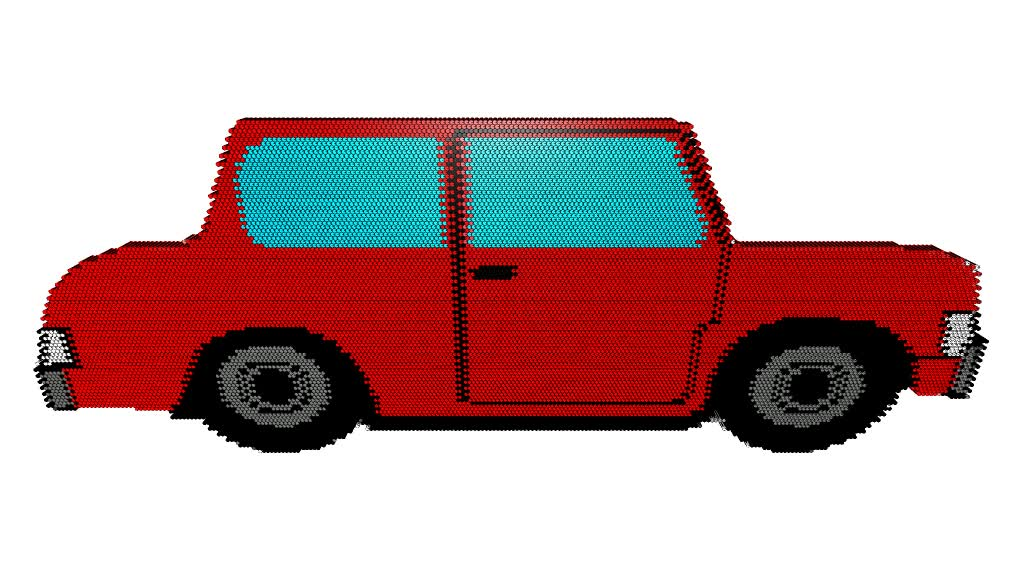
\includegraphics[width=\linewidth]{videos/5-scenario.jpg}}
		}
	\end{column} 
\end{columns}
\vspace{-0.5cm}
\item<4-> Research problems (proposed high-level primitives):
		\begin{enumerate}
			\item Shape construction
			\item Time synchronization
			\item Centrality-based leader election
		\end{enumerate}
\end{itemize}
}
\only<2-> {
	\begin{textblock*}{0.96\paperwidth}(0.02\paperwidth,0.88\paperheight)
		\tiny
		%\footnotesize 
	{
		\setstretch{0}
		\begin{center}			
			*Image based on modified versions of images released in the public domain under the Creative Commons CC0 license which were downloaded from \href{https://pixabay.com/fr/loupe-grossissant-transparent-303408/}{Pixabay} and  \href{http://fotomelia.com/?download=clipart-illustration-voiture-rouge-images-photos-gratuites}{Fotomelia}.
		\end{center}
	}
	\end{textblock*}
}
\end{frame}